\documentclass{article}

\usepackage[german]{babel}
\usepackage{array}
\usepackage[letterpaper,top=2cm,bottom=2cm,left=3cm,right=3cm,marginparwidth=1.75cm]{geometry}

\usepackage{amsmath}
\usepackage{graphicx}
\usepackage{subcaption} % Added package
\usepackage[colorlinks=true, allcolors=blue]{hyperref}
\usepackage[T1]{fontenc}
\usepackage{tabularx}
\usepackage{booktabs}


\title{Übungsprotokoll - NWG2 - Übung 05 \\ Link Aggregation}
\author{\vspace{0.5cm} Thomas Brandstetter (s2210239002) \& Jakob Mayr (s2210239021)}

\begin{document}
\maketitle

\section{Konfiguration der Endsysteme}

In der folgenden Übung haben wir die PCs 4.1 und 4.2 benutzt, somit sind die Netze 4.x verwendet worden. Die IP-Konfiguration wird folgendermaßen vergeben: Klick auf „Network“ in der Taskleiste $\rightarrow$ „Network \& Internet Settings“ $\rightarrow$ „Change adapter options“ $\rightarrow$ gewünschtes Netzwerk Interface auswählen, in diesem Fall Ethernet 2 $\rightarrow$ „Properties“ $\rightarrow$ Doppelklick auf „Internet Protocol Version 4“ bzw. „Internet Protocol Version 6“. In den geöffneten Fenstern können wir nun jeweils die IP-Adresse, Subnetzmaske/Präfix und das Gateway eingeben. Folglich sind die Konfigurationen beider PCs zu sehen:

\begin{figure}[!htp]
  \centering
  \begin{minipage}[b]{0.2\textwidth}
    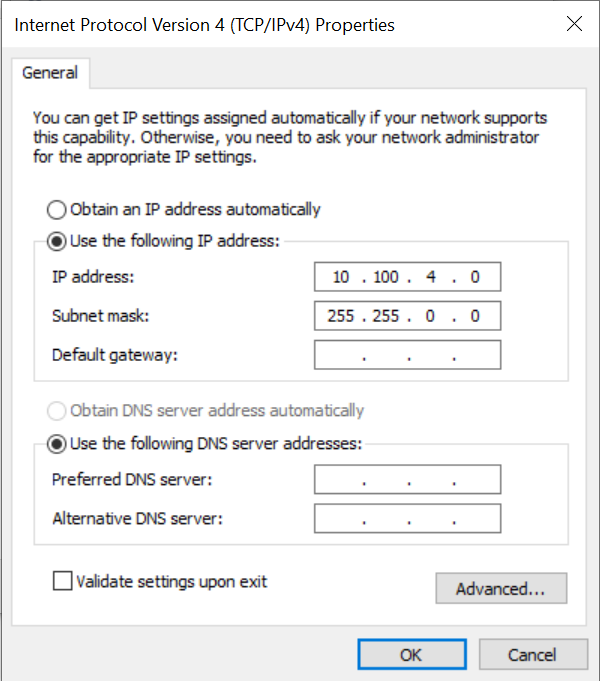
\includegraphics[width=\textwidth]{Arbeitsergebnisse/PC41/pc41_IPv4_config.png}
    \caption{PC41 IPv4 config}
  \end{minipage}
  \hspace{0.8cm}
  \begin{minipage}[b]{0.2\textwidth}
    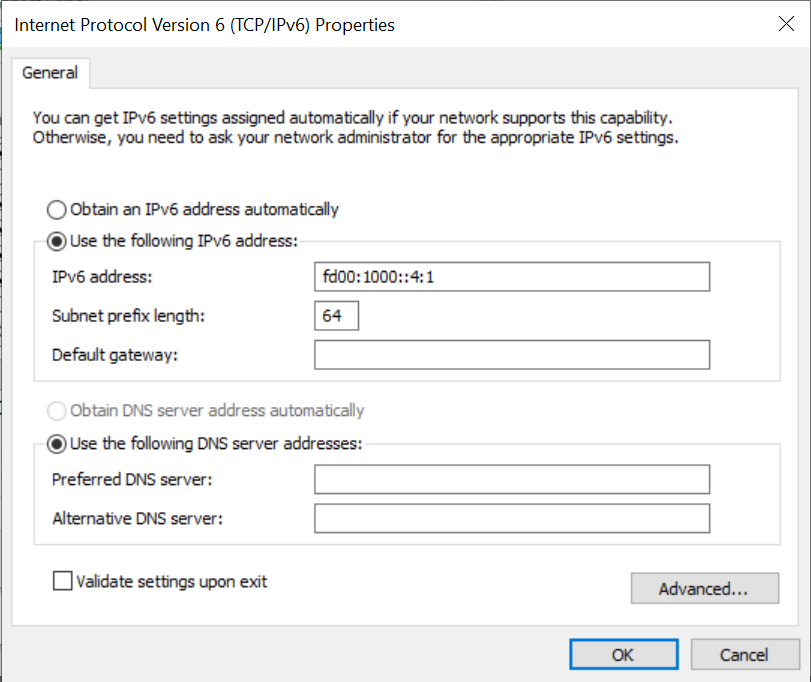
\includegraphics[width=\textwidth]{Arbeitsergebnisse/PC41/pc41_IPv6_config.png}
    \caption{PC41 IPv6 config}
  \end{minipage}
  \hspace{0.8cm}
  \begin{minipage}[b]{0.2\textwidth}
    \includegraphics[width=\textwidth]{Arbeitsergebnisse/PC42/pc42_IPv4_config.png}
    \caption{PC42 IPv4 config}
  \end{minipage}
  \hspace{0.8cm}
  \begin{minipage}[b]{0.2\textwidth}
    \includegraphics[width=\textwidth]{Arbeitsergebnisse/PC42/pc42_IPv6_config.png}
    \caption{PC42 IPv6 config}
  \end{minipage}
\end{figure}

\pagebreak



\section{Konfiguration des Gruppenrouters}

...\\

\begin{table}[htbp]
    \centering
    \begin{tabularx}{\textwidth}{|X|X|}
        \toprule
        \textbf{Befehl} & \textbf{Erklärung} \\
        \midrule
        ... & ...\\
        \hline
        ... & ...\\
        \bottomrule
    \end{tabularx}
    \caption{Verwendete Befehle zur Konfiguration des Gruppenrouters}
\end{table}

\noindent notes...



\section{Konfiguration der Gruppenswitches}

...\\

\begin{table}[htbp]
    \centering
    \begin{tabularx}{\textwidth}{|X|X|}
        \toprule
        \textbf{Befehl} & \textbf{Erklärung} \\
        \midrule
        ... & ...\\
        \hline
        ... & ...\\
        \bottomrule
    \end{tabularx}
    \caption{Verwendete Befehle zur Konfiguration der Gruppenswitches}
    \label{tab:commands}
\end{table}
\noindent notes...

\section{Fragen zur Konfiguration}

\subsection*{Frage 4.1 \normalfont Warum können ohne die Link Aggregation (das Erstellen der Channel Group) nicht beide Links verwendet werden?}
...\\

\subsection*{Frage 4.2 \normalfont Wie kann durch ein geeignetes Load Balancing sichergestellt werden, dass beide Rechner mit voller Geschwindigkeit bediengt werden?}
...\\

\subsection*{Frage 4.3 \normalfont Wenn Gruppe A die ACLs bereits fertig konfiguriert hat, Gruppe B aber nicht, wie wirkt sich das auf Ping zwischen den linken PCs aus? Falls es nicht geht, welche Fehlermeldungen erscheinen wann?}
...\\

\subsection*{Frage 4.4 \normalfont Wie wirken sich die ACLs auf den Kontakt zum FTP Server aus, und warum?} 
...\\

\subsection*{Frage 4.5 \normalfont Was bedeutet es für denk linken PC, dass er an einem Mirror Port hängt? Wie wirkt sich das auf seine Kommunkationsfähigkeit aus? Welche ports sollten für einen Mirror Port verwendet werden und warum?}
...\\

\pagebreak
\section{Tests und Interpretation ihrer Resultate}

\subsection{GS41 \& GS42}
Verwendete "Load-Balancing" Konfiguration auf des Switchtes GS41 und GS42:\\
\begin{figure}[!htp]
  \centering
  \begin{minipage}[b]{0.45\textwidth}
    \includegraphics[width=\textwidth]{Arbeitsergebnisse/GS41/GS41_etherchannel.png}
    \caption{GS41 EtherChannel Load-Balancing Configuration}
  \end{minipage}
  \hspace{0.8cm}
  \begin{minipage}[b]{0.45\textwidth}
    \includegraphics[width=\textwidth]{Arbeitsergebnisse/GS41/GS41_etherchannel.png}
    \caption{GS41 EtherChannel Load-Balancing Configuration}
  \end{minipage}
\end{figure}

\pagebreak
\subsection{PC41}
Ping von PC41 zu PC42, Ping zu Netz 8 - PC81 (fehlgeschlagen da ACL) und FTP-Verbindung\\
\begin{figure}[!htp]
  \centering
  \begin{minipage}[b]{0.25\textwidth}
    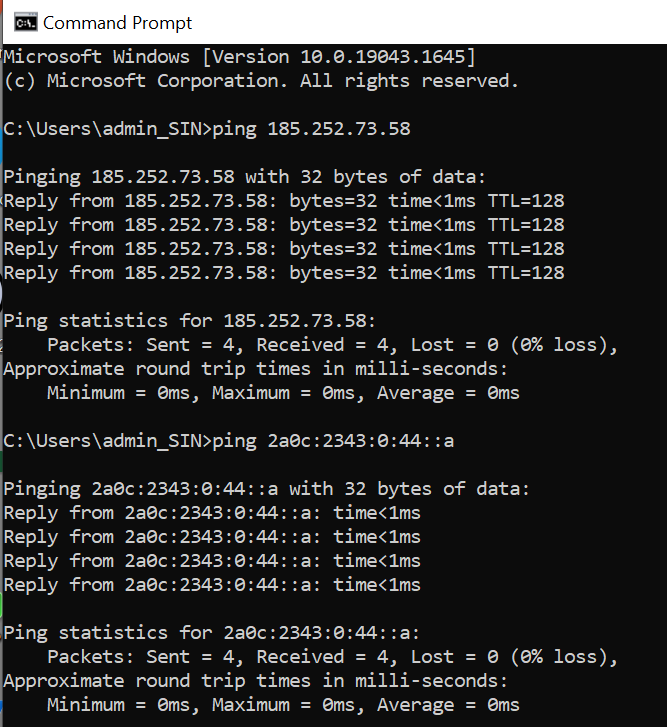
\includegraphics[width=\textwidth]{Arbeitsergebnisse/PC41/pc41_ping_pc42.png}
    \caption{PC41 ping PC42}
  \end{minipage}
  \hspace{0.8cm}
  \begin{minipage}[b]{0.25\textwidth}
    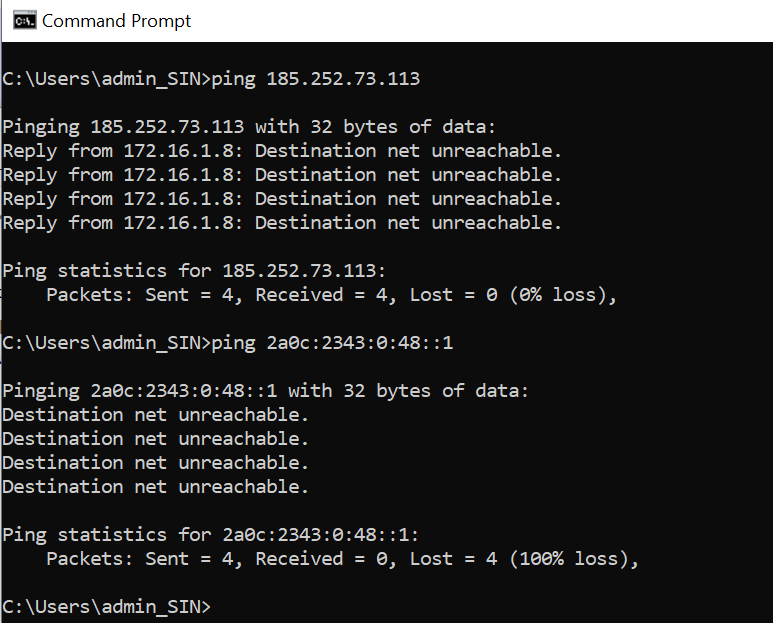
\includegraphics[width=\textwidth]{Arbeitsergebnisse/PC41/pc41_ping_failed.png}
    \caption{PC41 Ping zu Netz 8 - PC81 (fehlgeschlagen da ACL)}
  \end{minipage}
  \hspace{0.8cm}
  \begin{minipage}[b]{0.25\textwidth}
    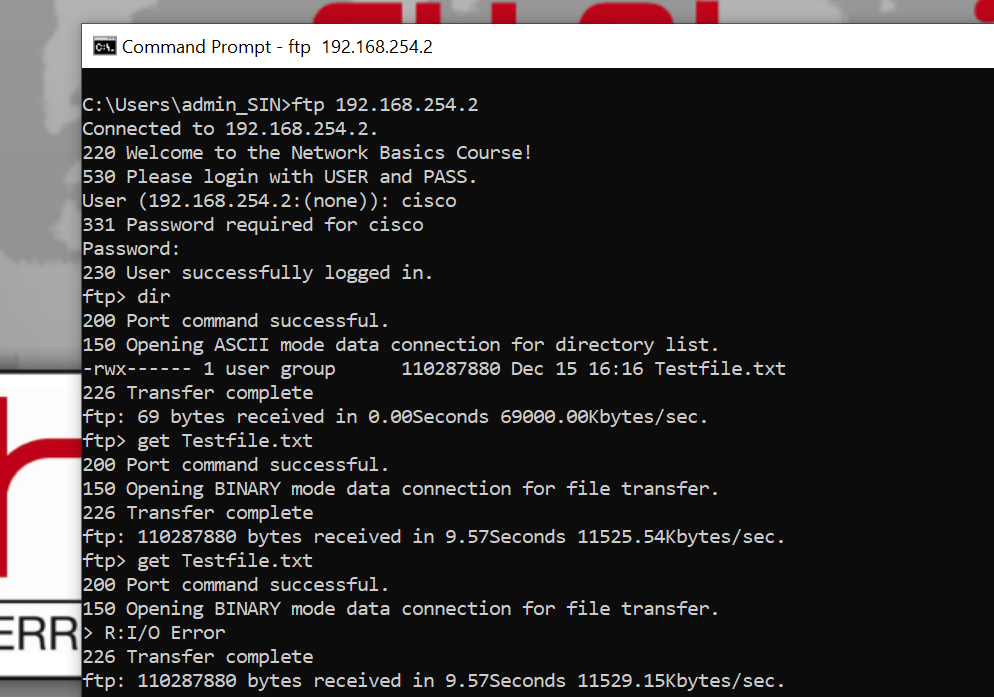
\includegraphics[width=\textwidth]{Arbeitsergebnisse/PC41/pc41_ftp.png}
    \caption{PC41 FTP-Verbindung}
  \end{minipage}
\end{figure}

\subsection{PC42}
Ping von PC42 zu PC41, Ping zu Netz 8 - PC82 (fehlgeschlagen da ACL) und FTP-Verbindung\\
\begin{figure}[!htp]
  \centering
  \begin{minipage}[b]{0.25\textwidth}
    \includegraphics[width=\textwidth]{Arbeitsergebnisse/PC42/pc42_ping_PC41.png}
    \caption{PC42 ping PC41}
  \end{minipage}
  \hspace{0.8cm}
  \begin{minipage}[b]{0.25\textwidth}
    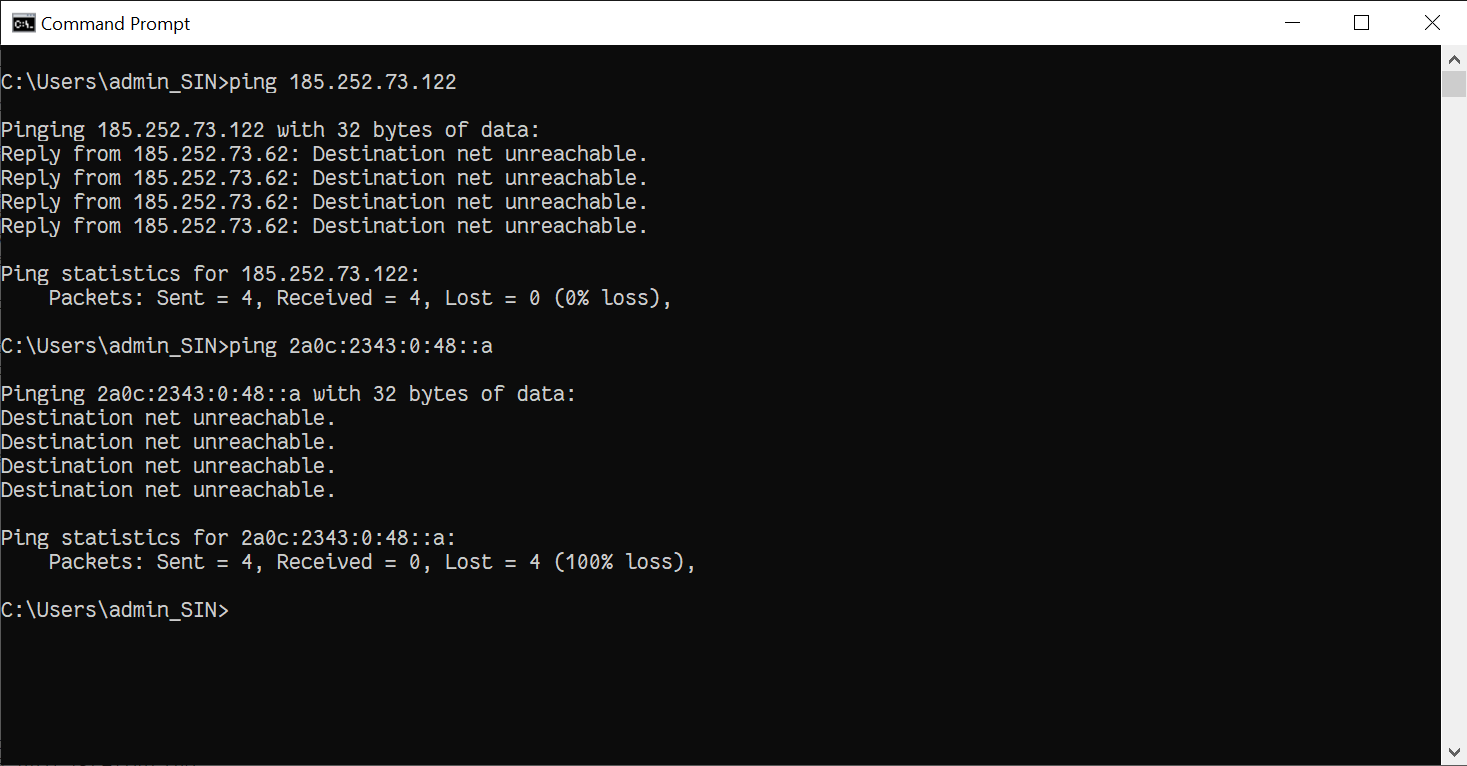
\includegraphics[width=\textwidth]{Arbeitsergebnisse/PC42/pc42_ping_failed.png}
    \caption{PC42 Ping zu Netz 8 - PC82 (fehlgeschlagen da ACL)}
  \end{minipage}
  \hspace{0.8cm}
  \begin{minipage}[b]{0.25\textwidth}
    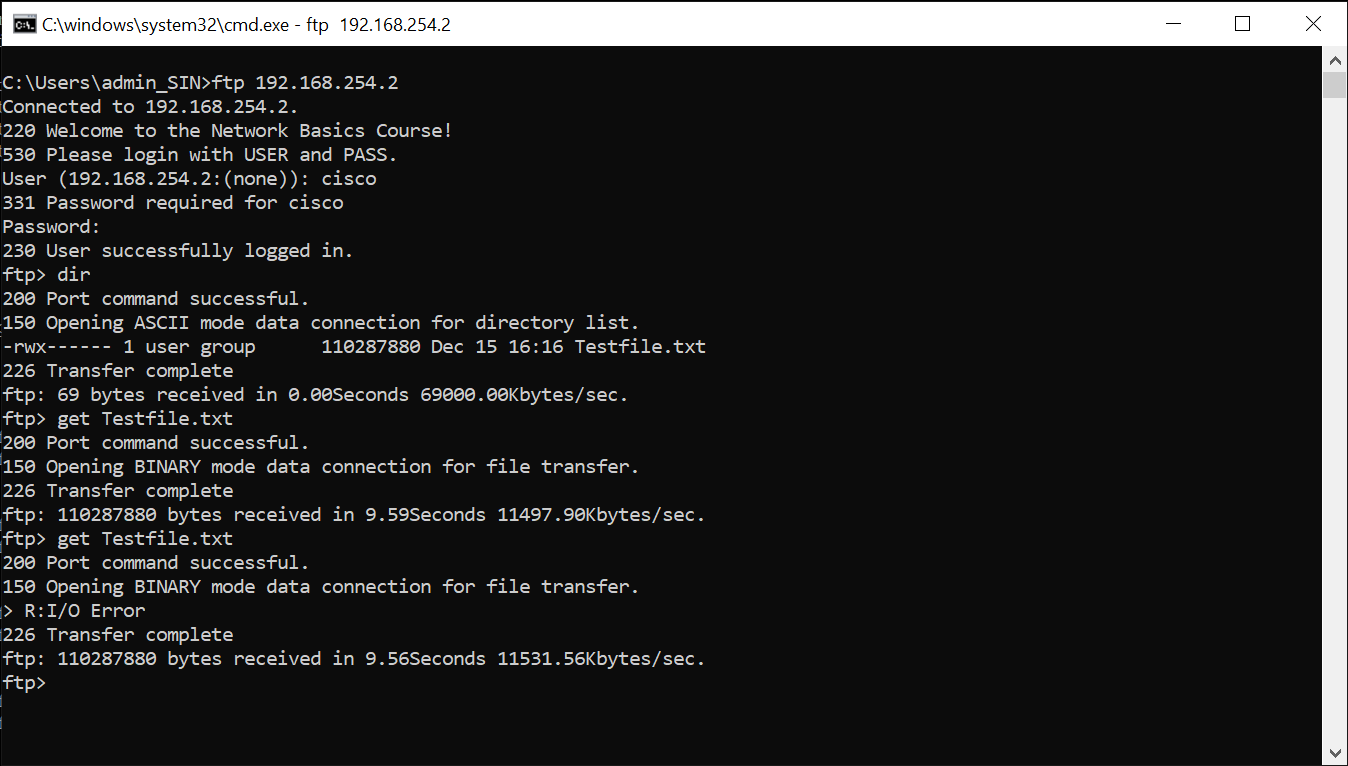
\includegraphics[width=\textwidth]{Arbeitsergebnisse/PC42/pc42_ftp.png}
    \caption{PC42 FTP-Verbindung}
  \end{minipage}
\end{figure}

\end{document}

